\begin{enumerate}[label=\arabic*.,ref=\theenumi]
\item 	The state diagram of a sequence detector is shown in
  \figref{fig:gate/ec/2020/39/1}.
		 State $S_0$ is the initial state of the sequence detector. If the output is 1, then
\hfill (GATE EC 2020)
\begin{enumerate}
 \item the sequence 01010 is detected
 \item the sequence 01011 is detected
 \item the sequence 01110 is detected
 \item the sequence 01001 is detected	 
\end{enumerate}	
	\begin{figure}[H]
    \centering
    \resizebox{0.75\columnwidth}{!}{%
  \input{gate/ec/2020/39/figs/diagram.tex}
		}
  \caption{}
  \label{fig:gate/ec/2020/39/1}		
  \end{figure}	 
\item A sequence detector is designed to detect precisely 3 digital inputs, with overlapping sequences detectable. For the sequence $(1,0,1)$ and input data $(1,1,0,1,0,0,1,1,0,1,0,1,1,0)$, what is the output of this detector?
		\begin{enumerate}
			\item 1,1,0,0,0,0,1,1,0,1,0,0
			\item 0,1,0,0,0,0,0,1,0,1,0,0
			\item 0,1,0,0,0,0,0,1,0,1,1,0
			\item 0,1,0,0,0,0,0,0,1,0,0,0
		\end{enumerate}
		\hfill (GATE EE 2020)
\item Consider a $3$-bit counter, designed using T flip-flops, as shown below
in \figref{fig:3bitcounter.jpg}.
Assuming the initial state of the counter given by $PQR$ as $000$,what are the next three states?
                 \hfill(GATE CS 2021)
\begin{enumerate}
\item $011, 101, 000$
\item $010, 101, 000$
\item $010, 101, 000$
\item $010, 101, 000$
\end{enumerate}
     \begin{figure}[H]
\centering
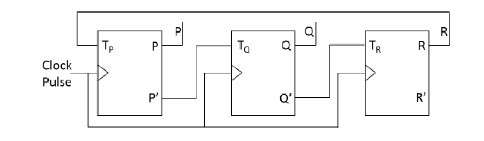
\includegraphics[width=0.75\columnwidth]{ide/fsm/figs/3bitcounter.jpg}
\caption{}
\label{fig:3bitcounter.jpg}
\end{figure}
%
\item The state transition diagram for the circuit shown in 
	\figref{fig:GATE IN2019,39}
	is
                         \hfill(GATE IN 2019)
\begin{figure}[H]
\centering
    \resizebox{0.5\columnwidth}{!}{%
\begin{circuitikz}
            \draw (2,2)coordinate(w)--(5,2)coordinate(x)--(5,6)coordinate(x)--(2,6)coordinate(z)--(2,2)coordinate(w);
            \draw (0.85,5.5)--(2,5.5);
            \draw (2,5.5)node[right]{$D$};
            \draw (1,0)--(1,2.5)--(2,2.5);
            \draw (1,-0.5)node[]{$CLK$};
            \draw (2,2.25)--(2.3,2.5)--(2,2.75);
            \draw (5,5.5)node[left]{$Q$}--(8,5.5)node[right]{$1$};
            \draw (5,2.5)node[left]{$\overline{Q}$}--(8,2.5)node[right]{$0$};
              % Reversed NAND gate (horizontally flipped)
    \draw (5,8) node[nand port,scale=-1] (nand) {};
    %\draw (nand.in 1) node[left] {};
%\draw (nand.in 2) node[left] {};
    
    % Output
    
    \draw (nand.out) -- ++(-4,0) -- ++(0,-2.5) node[above]{};
    % Inputs
    \draw (nand.in 1) -- ++(0,-2.2) node[below]{};
    \draw (nand.in 2) -- ++(4,0)--++(0,-4.2)--++(-0.86,0) node[below]{};
    \draw (8,2)--(8,6)--(9.5,5)--(9.5,3)--(8,2);
    \draw [->](9,0)node[right]{$A$}--(9,2.7);
    
\end{circuitikz}

	}
    \caption{}
	\label{fig:GATE IN2019,39}
\end{figure}
%
\begin{enumerate}
%% options1
\item 
	\figref{fig:GATE IN2019,39-1}
\begin{figure}[H]
\centering
    \resizebox{0.5\columnwidth}{!}{%
\begin{circuitikz}
[-latex ,node distance=4cm and 2cm,thick,state/.style={circle,draw, minimum width =1cm}] 

\node[state] (Q0) {$Q=0$};
\node[state] (Q1) [right of=Q0]{$Q=1$};
\path (Q0) edge [bend left] node [above=0.15] {A = 1} (Q1);
\path (Q0) edge [loop above ,out=100 ,in=150,distance=2cm] node {A = 0} (Q0);
\path  (Q1) edge [bend left] node [below=0.15] {A = 1} (Q0);
\path (Q1) edge [loop above ,in=60,out=120,distance=2cm] node {A=0} (Q1);
        
\end{circuitikz}


	}
    \caption{}
	\label{fig:GATE IN2019,39-1}
\end{figure}
%% options2
\item 
	\figref{fig:GATE IN2019,39-2}
\begin{figure}[H]
\centering
    \resizebox{0.5\columnwidth}{!}{%
\begin{circuitikz}[-latex ,node distance=4cm and 2cm,thick,state/.style={circle,draw, minimum width =1cm}]
\node[state] (Q0) {$Q=0$};
\node[state] (Q1) [right of=Q0]{$Q=1$};
\path (Q0) edge [bend left] node [above=0.15] {A = 1} (Q1);
\path  (Q1) edge [bend left] node [above=0.15] {A = 1} (Q0);
\path (Q0) edge [loop above ,out=100,in=150,distance=2cm] node {A = 0} (Q0);
\path (Q1) edge [bend left ,out=85,in=90] node [above=0.15] {A = 0} (Q0);
\end{circuitikz}


	}
    \caption{}
	\label{fig:GATE IN2019,39-2}
\end{figure}
\item 
	\figref{fig:GATE IN2019,39-3}
\begin{figure}[H]
\centering
    \resizebox{0.5\columnwidth}{!}{%
\begin{circuitikz}
[-latex ,node distance=4cm and 2cm,thick,state/.style={circle,draw, minimum width =1cm}]

\node[state] (Q0) {$Q=0$};
\node[state] (Q1) [right of=Q0]{$Q=1$};
\path (Q0) edge [bend left] node [above=0.15] {A = 1} (Q1);
\path  (Q1) edge [bend left] node [above=0.15] {A = 1} (Q0);
\path (Q1) edge [loop above ,in=20,out=70,distance=2cm] node {A = 0} (Q1);
\path (Q0) edge [bend left ,out=85,in=90] node [above=0.15] {A = 0} (Q1);  
\end{circuitikz}


	}
    \caption{}
	\label{fig:GATE IN2019,39-3}
\end{figure}
\item 
	\figref{fig:GATE IN2019,39-4}
\begin{figure}[H]
\centering
    \resizebox{0.5\columnwidth}{!}{%
\begin{circuitikz}[-latex ,node distance=4cm and 2cm,thick,state/.style={circle,draw, minimum width =1cm}]
\node[state] (Q0) {$Q=0$};
\node[state] (Q1) [right of=Q0]{$Q=1$};
\path (Q0) edge [bend left] node [above=0.15] {A = 0} (Q1);
\path (Q0) edge [loop above ,out=100 ,in=150,distance=2cm] node {A = 1} (Q0);
\path  (Q1) edge [bend left] node [below=0.15] {A = 1} (Q0);
\path (Q1) edge [loop above ,in=60,out=120,distance=2cm] node {A=0} (Q1);
\end{circuitikz}


	}
    \caption{}
	\label{fig:GATE IN2019,39-4}
\end{figure}
%
\end{enumerate}
%
\iffalse
\item A sequence detector is designed to detect precisely $3$ digital inputs, with overlapping sequences detectable. For the sequence $\brak{1,0,1}$ and input data $\brak{1,1,0,1,0,0,1,1,0,1,0,1,1,0}$, the output sequence is
$\hfill\brak{GATE\enspace EE2020-15}$
   \begin{enumerate}
  \item  $\brak{1,1,0,0,0,0,1,1,0,1,0,0}$
  \item $\brak{0,1,0,0,0,0,0,1,0,1,0,0}$
  \item $\brak{0,1,0,0,0,0,0,1,0,1,1,0}$
  \item $\brak{0,1,0,0,0,0,0,0,1,0,0,0}$

\end{enumerate}
\fi
%
\item A finite state machine (FSM) is implemented using the D flip-flops $A$ and $B$, and logic gates, as shown in  
\figref{fig:ide/fsm/figs/circuit}
	below. The four possible states of the FSM are $Q_AQ_B = 00, 01, 10$ and	 $11$.  
Assume that $X_{IN}$ is held at a constant logic level throughout the operation of the FSM. When the FSM is initialized to the state $Q_AQ_B = 00$ and clocked, after a few clock cycles, it starts cycling through
\hfill{(GATE EC 2017)}
\begin{enumerate}
\item all of the four possible states if $X_{in} = 1$
\item three of the four possible states if $X_{in} = 0$
\item only two of the four possible states if $X_{in} = 1$
\item only two of the four possible states if $X_{in} = 0$
\end{enumerate}
%
\begin{figure}[H]
\centering
\resizebox{0.75\columnwidth}{!}{%
	\begin{circuitikz}
\tikzstyle{every node}=[font=\Large]

\draw [, line width=0.9pt](4,6) to[short] (17,6);
\draw (4,6) to[short] (17,6);
\draw [, line width=0.9pt ] (5,7) rectangle (9,11);
\draw [, line width=0.9pt ] (15,7) rectangle (19,11);
\draw (11,10) to[short] (11.5,10);
\draw (11,9.5) to[short] (11.5,9.5);
\draw (11.5,10) node[ieeestd nand port, anchor=in 1, scale=0.89](port){} (port.out) to[short] (13.5,9.75);
\draw [, line width=0.9pt](11,9.5) to[short] (11,8.75);
\draw [, line width=0.9pt](9,10) to[short] (11,10);
\draw [, line width=0.9pt](13.5,9.75) to[short] (14,9.75);
\draw [, line width=0.9pt](14,9.75) to[short] (14,10);
\draw [, line width=0.9pt](14,10) to[short] (15,10);
\draw [, line width=0.9pt](19,10) to[short] (20.5,10);
\draw [, line width=0.9pt](20,10) to[short] (20,12);
\draw [, line width=0.9pt](20,12) to[short] (20,13);
\draw[, line width=0.9pt] (20,13) to[short] (10,13);
\draw [, line width=0.9pt](10,10) to[short] (10,12);
\draw (9,13) to[short] (8.75,13);
\draw (9,12.5) to[short] (8.75,12.5);
\draw (8.75,13) node[ieeestd xor port, anchor=in 2, scale=0.89, rotate=180](port){} (port.out) to[short] (6.75,12.75);
\draw[, line width=0.9pt] (10,13) to[short] (8.75,13);
\draw [, line width=0.9pt](10,12) to[short] (10,12.5);
\draw[, line width=0.9pt] (10,12.5) to[short] (9,12.5);
\draw[, line width=0.9pt] (6.75,12.75) to[short] (4,12.75);
\draw [, line width=0.9pt](4,12.75) to[short] (4,10);
\draw [, line width=0.9pt](4,10) to[short] (5,10);
\node [font=\Large] at (7,9) {A};
\node [font=\Large] at (17,9) {B};
\node [font=\Large] at (5.25,10) {D};
\node [font=\Large] at (15.25,10) {D};
\node [font=\Large] at (18.5,10) {Q};
\node [font=\Large] at (8.5,10) {Q};
\node [font=\Large] at (8.5,8) {$\bar Q$};
\node [font=\Large] at (18.5,8) {$\bar Q$};
\node [font=\Large] at (6,7.75) {CK};
\node [font=\Large] at (16,8) {CK};
\node [font=\Large] at (3.25,6) {CLK};
\node [font=\Large] at (11,8.5) {Xin};
\draw [, line width=0.9pt](6.75,6) to[short] (6.75,7);
\draw [, line width=0.9pt](17,6) to[short] (17,7);
\draw [line width=0.9pt, short] (6.25,7) -- (6.75,7.75);
\draw [line width=0.9pt, short] (6.75,7.75) -- (7.25,7);
\draw [line width=0.9pt, short] (16.5,7) -- (17,7.75);
\draw [line width=0.9pt, short] (17,7.75) -- (17.5,7);
\node [font=\Large] at (11.5,10.5) {$Q_A$};
\node [font=\Large] at (20.25,9.5) {$Q_B$};
\end{circuitikz}

}%
	\caption{}
\label{fig:ide/fsm/figs/circuit}
\end{figure}
\iffalse
\item For the given digital circuit
in	\figref{fig:Image},
	 $A = B = 1$. Assume that AND, OR, and NOT gates have propagation delays of $10\mathrm{ns}$,$10\mathrm{ns}$, and $5\mathrm{ns}$ respectively. All lines have zero
propagation delay. Given that $C = 1$ when the circuit is turned on, the frequency of steady-state oscillation of the output $Y$  is  \rule{1cm}{0.5pt}.
\hfill (GATE IN 2023)
\begin{figure}[H]
        \centering  
        
        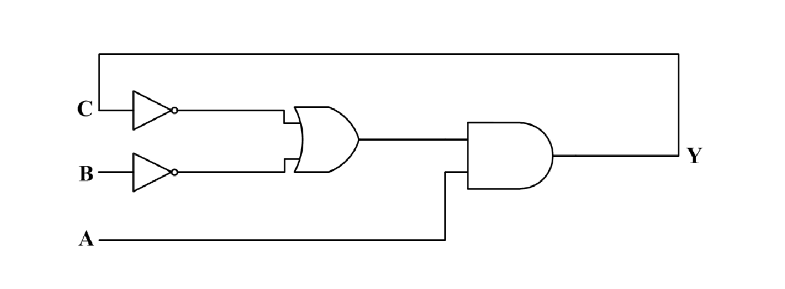
\includegraphics[width=0.75\columnwidth]{figs/gate.png}
        \caption{Image}
	\label{fig:Image}
\end{figure}
%
\item In the circuit diagram shown below
in \figref{fig:GATE Digram}, the logic gates operate with a supply voltage of $1 V$. NAND and XNOR have $200$ps and $400$ps input-to-output delay, respectively.

At time $t=T.A(t)=0,B(t)=1 and Z(t)=0.$ When the inputs are changed to $A(t)=1,B(t)=0 \text{at} t=2T$, a 1 V pulse is observed at $Z$. the pulse width of the $1 V$ pulse is  ps.


\hfill{(GATE BM 2022)}

\begin{figure}[H]
\centering
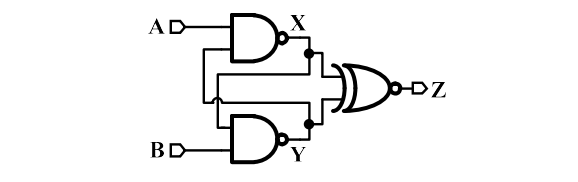
\includegraphics[width=0.75\columnwidth]{figs/bm2022.png}
\caption{}
\label{fig:GATE Digram}
\end{figure}

\begin{enumerate}
\item $100$
\item $200$
\item $400$
\item $600$
\end {enumerate}
%
\fi
\item Find the states in 
	\figref{fig:GATEEC2020-50}.
\hfill (GATE EC 2020)
%
	\begin{figure}[H]
    \centering
    \resizebox{0.75\columnwidth}{!}{%
    \begin{circuitikz}
    % Universal Flip-flop with custom pin names
    \draw (3,-8.5) node[flipflop,external pins width=0, name=FF1,scale=1.2] {};
    
    % Custom pin names
    \node [right,font=] at (FF1.bpin 1) {\textsl{}};
    \node [left,font=] at (3.8,-7.8) {};
    \node [left,font=] at (4,-8.2) {};
    \node [left,font=] at (4,-8.6) {};
    \node [left,font=] at (0.8,-9.3) {\textsl{Clk}};
    \draw (FF1.west) ++(0,-0.8) -- ++(0.2,-0.2) -- ++(-0.2,-0.2) -- cycle;
    \draw (FF1.pin 3) -- ++(-1.45,0);
    \draw (-0.8,-10.2) -- ++ (0.5,0)-- ++ (0,0.5) -- ++(0.5,0)-- ++(0,-0.5)-- ++ (0.5,0) -- ++ (0,0.5)-- ++(0.5,0)-- ++(0,-0.5);
    
    
    \draw (3,-13) node[flipflop, name=FF2,scale=1.2] {};
    
    % Custom pin names
    \node [right,font=] at (FF2.bpin 1) {\textsl{}};
    \node [right,font=] at (FF1.bpin 1) {\textsl{}};
    \node [left,font=] at (3.8,-12.4) {};
    \node [left,font=] at (4,-12.8) {};
    \node [left,font=] at (4,-13.2) {};
    \node [left,font=] at (3.8,-11.3) {$\text{Flip Flop2}$};
    \node [left,font=] at (3.8,-6.8) {$\text{Flip Flop1}$};

    \draw (FF2.west) ++(0,-0.8) -- ++(0.2,-0.2) -- ++(-0.2,-0.2) -- cycle;
    \node[ieeestd nand port] (NAND) at (9.5,-8.3) {};
    \node[ieeestd xor port] (xor) at (7,-8.0) {};
    
    \draw (FF1.pin 6) -- ++(0.8,0) to[bend right](5.2,-7.5) -- ++ (0.25,0) -- ++ (0,-0.22) -- ++ (0.6,0);
    \node [left,font=] at (10.0,-7.5) {};
    \node [left,font=] at (7.7,-7) {};
    \draw (FF1.pin 1) -- ++(-2,0) -- ++ (0,1.5) -- ++ (5,0) -- ++ (0,-6) -- ++ (-1,0) ;
    %\draw (2,-12) -- ++(-2,0) -- ++ (0,-3) -- ++ (6,0) -- ++ (0,5) -| (NAND.out) ;
    \draw (xor.in 2)-- ++(0,-1)-|(NAND.in 2);
    \draw (xor.out)--(xor.out) -|(NAND.in 1);
    \draw (6,-9.27)-- ++(-0.3,0) node[left]{IN};
    \draw (FF1.pin 6) -- ++(0.8,0) to[bend right](5.2,-7.5) -- ++ (0.25,0) -- ++ (0,-0.22) -- ++ (0.6,0);
    \draw (1.4,-9.5) -- ++ (0,-4.5);
    \draw (2.0,-14) -- ++(-0.6,0);
    \draw (2,-12) -- ++(-0.4,0) to[bend left](1.2,-12) -- ++ (-1,0) -- ++ (0,-4) -- ++ (11,0)-- ++(0,8) -|(NAND.out);

\end{circuitikz}

	}
    \caption{}
	\label{fig:GATEEC2020-50}
\end{figure}

\end{enumerate}
